\documentclass[1p]{elsarticle_modified}
%\bibliographystyle{elsarticle-num}

%\usepackage[colorlinks]{hyperref}
%\usepackage{abbrmath_seonhwa} %\Abb, \Ascr, \Acal ,\Abf, \Afrak
\usepackage{amsfonts}
\usepackage{amssymb}
\usepackage{amsmath}
\usepackage{amsthm}
\usepackage{scalefnt}
\usepackage{amsbsy}
\usepackage{kotex}
\usepackage{caption}
\usepackage{subfig}
\usepackage{color}
\usepackage{graphicx}
\usepackage{xcolor} %% white, black, red, green, blue, cyan, magenta, yellow
\usepackage{float}
\usepackage{setspace}
\usepackage{hyperref}

\usepackage{tikz}
\usetikzlibrary{arrows}

\usepackage{multirow}
\usepackage{array} % fixed length table
\usepackage{hhline}

%%%%%%%%%%%%%%%%%%%%%
\makeatletter
\renewcommand*\env@matrix[1][\arraystretch]{%
	\edef\arraystretch{#1}%
	\hskip -\arraycolsep
	\let\@ifnextchar\new@ifnextchar
	\array{*\c@MaxMatrixCols c}}
\makeatother %https://tex.stackexchange.com/questions/14071/how-can-i-increase-the-line-spacing-in-a-matrix
%%%%%%%%%%%%%%%

\usepackage[normalem]{ulem}

\newcommand{\msout}[1]{\ifmmode\text{\sout{\ensuremath{#1}}}\else\sout{#1}\fi}
%SOURCE: \msout is \stkout macro in https://tex.stackexchange.com/questions/20609/strikeout-in-math-mode

\newcommand{\cancel}[1]{
	\ifmmode
	{\color{red}\msout{#1}}
	\else
	{\color{red}\sout{#1}}
	\fi
}

\newcommand{\add}[1]{
	{\color{blue}\uwave{#1}}
}

\newcommand{\replace}[2]{
	\ifmmode
	{\color{red}\msout{#1}}{\color{blue}\uwave{#2}}
	\else
	{\color{red}\sout{#1}}{\color{blue}\uwave{#2}}
	\fi
}

\newcommand{\Sol}{\mathcal{S}} %segment
\newcommand{\D}{D} %diagram
\newcommand{\A}{\mathcal{A}} %arc


%%%%%%%%%%%%%%%%%%%%%%%%%%%%%5 test

\def\sl{\operatorname{\textup{SL}}(2,\Cbb)}
\def\psl{\operatorname{\textup{PSL}}(2,\Cbb)}
\def\quan{\mkern 1mu \triangleright \mkern 1mu}

\theoremstyle{definition}
\newtheorem{thm}{Theorem}[section]
\newtheorem{prop}[thm]{Proposition}
\newtheorem{lem}[thm]{Lemma}
\newtheorem{ques}[thm]{Question}
\newtheorem{cor}[thm]{Corollary}
\newtheorem{defn}[thm]{Definition}
\newtheorem{exam}[thm]{Example}
\newtheorem{rmk}[thm]{Remark}
\newtheorem{alg}[thm]{Algorithm}

\newcommand{\I}{\sqrt{-1}}
\begin{document}

%\begin{frontmatter}
%
%\title{Boundary parabolic representations of knots up to 8 crossings}
%
%%% Group authors per affiliation:
%\author{Yunhi Cho} 
%\address{Department of Mathematics, University of Seoul, Seoul, Korea}
%\ead{yhcho@uos.ac.kr}
%
%
%\author{Seonhwa Kim} %\fnref{s_kim}}
%\address{Center for Geometry and Physics, Institute for Basic Science, Pohang, 37673, Korea}
%\ead{ryeona17@ibs.re.kr}
%
%\author{Hyuk Kim}
%\address{Department of Mathematical Sciences, Seoul National University, Seoul 08826, Korea}
%\ead{hyukkim@snu.ac.kr}
%
%\author{Seokbeom Yoon}
%\address{Department of Mathematical Sciences, Seoul National University, Seoul, 08826,  Korea}
%\ead{sbyoon15@snu.ac.kr}
%
%\begin{abstract}
%We find all boundary parabolic representation of knots up to 8 crossings.
%
%\end{abstract}
%\begin{keyword}
%    \MSC[2010] 57M25 
%\end{keyword}
%
%\end{frontmatter}

%\linenumbers
%\tableofcontents
%
\newcommand\colored[1]{\textcolor{white}{\rule[-0.35ex]{0.8em}{1.4ex}}\kern-0.8em\color{red} #1}%
%\newcommand\colored[1]{\textcolor{white}{ #1}\kern-2.17ex	\textcolor{white}{ #1}\kern-1.81ex	\textcolor{white}{ #1}\kern-2.15ex\color{red}#1	}

{\Large $\underline{12a_{0072}~(K12a_{0072})}$}

\setlength{\tabcolsep}{10pt}
\renewcommand{\arraystretch}{1.6}
\vspace{1cm}\begin{tabular}{m{100pt}>{\centering\arraybackslash}m{274pt}}
\multirow{5}{120pt}{
	\centering
	\includegraphics[width=112pt]{../../../GIT/diagram.site/Diagrams/png/873_12a_0072.png}\\
\ \ \ A knot diagram\footnotemark}&
\allowdisplaybreaks
\textbf{Linearized knot diagam} \\
\cline{2-2}
 &
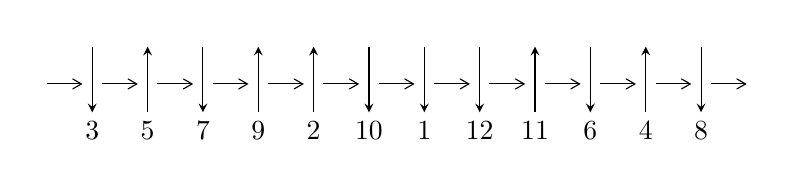
\begin{tikzpicture}[x=20pt, y=17pt]
	% nodes
	\node (C0) at (0, 0) {};
	\node (C1) at (1, 0) {};
	\node (C1U) at (1, +1) {};
	\node (C1D) at (1, -1) {3};

	\node (C2) at (2, 0) {};
	\node (C2U) at (2, +1) {};
	\node (C2D) at (2, -1) {5};

	\node (C3) at (3, 0) {};
	\node (C3U) at (3, +1) {};
	\node (C3D) at (3, -1) {7};

	\node (C4) at (4, 0) {};
	\node (C4U) at (4, +1) {};
	\node (C4D) at (4, -1) {9};

	\node (C5) at (5, 0) {};
	\node (C5U) at (5, +1) {};
	\node (C5D) at (5, -1) {2};

	\node (C6) at (6, 0) {};
	\node (C6U) at (6, +1) {};
	\node (C6D) at (6, -1) {10};

	\node (C7) at (7, 0) {};
	\node (C7U) at (7, +1) {};
	\node (C7D) at (7, -1) {1};

	\node (C8) at (8, 0) {};
	\node (C8U) at (8, +1) {};
	\node (C8D) at (8, -1) {12};

	\node (C9) at (9, 0) {};
	\node (C9U) at (9, +1) {};
	\node (C9D) at (9, -1) {11};

	\node (C10) at (10, 0) {};
	\node (C10U) at (10, +1) {};
	\node (C10D) at (10, -1) {6};

	\node (C11) at (11, 0) {};
	\node (C11U) at (11, +1) {};
	\node (C11D) at (11, -1) {4};

	\node (C12) at (12, 0) {};
	\node (C12U) at (12, +1) {};
	\node (C12D) at (12, -1) {8};
	\node (C13) at (13, 0) {};

	% arrows
	\draw[->,>={angle 60}]
	(C0) edge (C1) (C1) edge (C2) (C2) edge (C3) (C3) edge (C4) (C4) edge (C5) (C5) edge (C6) (C6) edge (C7) (C7) edge (C8) (C8) edge (C9) (C9) edge (C10) (C10) edge (C11) (C11) edge (C12) (C12) edge (C13) ;	\draw[->,>=stealth]
	(C1U) edge (C1D) (C2D) edge (C2U) (C3U) edge (C3D) (C4D) edge (C4U) (C5D) edge (C5U) (C6U) edge (C6D) (C7U) edge (C7D) (C8U) edge (C8D) (C9D) edge (C9U) (C10U) edge (C10D) (C11D) edge (C11U) (C12U) edge (C12D) ;
	\end{tikzpicture} \\
\hhline{~~} \\& 
\textbf{Solving Sequence} \\ \cline{2-2} 
 &
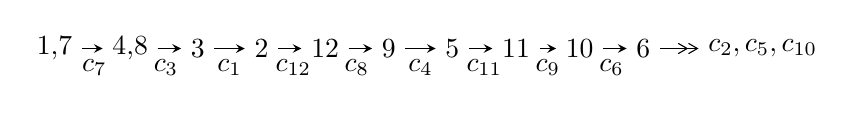
\begin{tikzpicture}[x=23pt, y=7pt]
	% node
	\node (A0) at (-1/8, 0) {1,7};
	\node (A1) at (17/16, 0) {4,8};
	\node (A2) at (17/8, 0) {3};
	\node (A3) at (25/8, 0) {2};
	\node (A4) at (33/8, 0) {12};
	\node (A5) at (41/8, 0) {9};
	\node (A6) at (49/8, 0) {5};
	\node (A7) at (57/8, 0) {11};
	\node (A8) at (65/8, 0) {10};
	\node (A9) at (73/8, 0) {6};
	\node (C1) at (1/2, -1) {$c_{7}$};
	\node (C2) at (13/8, -1) {$c_{3}$};
	\node (C3) at (21/8, -1) {$c_{1}$};
	\node (C4) at (29/8, -1) {$c_{12}$};
	\node (C5) at (37/8, -1) {$c_{8}$};
	\node (C6) at (45/8, -1) {$c_{4}$};
	\node (C7) at (53/8, -1) {$c_{11}$};
	\node (C8) at (61/8, -1) {$c_{9}$};
	\node (C9) at (69/8, -1) {$c_{6}$};
	\node (A10) at (11, 0) {$c_{2},c_{5},c_{10}$};

	% edge
	\draw[->,>=stealth]	
	(A0) edge (A1) (A1) edge (A2) (A2) edge (A3) (A3) edge (A4) (A4) edge (A5) (A5) edge (A6) (A6) edge (A7) (A7) edge (A8) (A8) edge (A9) ;
	\draw[->>,>={angle 60}]	
	(A9) edge (A10);
\end{tikzpicture} \\ 

\end{tabular} \\

\footnotetext{
The image of knot diagram is generated by the software ``\textbf{Draw programme}" developed by Andrew Bartholomew(\url{http://www.layer8.co.uk/maths/draw/index.htm\#Running-draw}), where we modified some parts for our purpose(\url{https://github.com/CATsTAILs/LinksPainter}).
}\phantom \\ \newline 
\centering \textbf{Ideals for irreducible components\footnotemark of $X_{\text{par}}$} 
 
\begin{align*}
I^u_{1}&=\langle 
-6.32959\times10^{206} u^{99}+1.69512\times10^{207} u^{98}+\cdots+6.75897\times10^{206} b+1.91806\times10^{207},\\
\phantom{I^u_{1}}&\phantom{= \langle  }-1.41888\times10^{207} u^{99}+4.03733\times10^{207} u^{98}+\cdots+1.35179\times10^{207} a+1.32866\times10^{207},\\
\phantom{I^u_{1}}&\phantom{= \langle  }u^{100}-3 u^{99}+\cdots-3 u+1\rangle \\
I^u_{2}&=\langle 
b-2 a,\;9 a^2+3 a+1,\;u-1\rangle \\
\\
\end{align*}
\raggedright * 2 irreducible components of $\dim_{\mathbb{C}}=0$, with total 102 representations.\\
\footnotetext{All coefficients of polynomials are rational numbers. But the coefficients are sometimes approximated in decimal forms when there is not enough margin.}
\newpage
\renewcommand{\arraystretch}{1}
\centering \section*{I. $I^u_{1}= \langle -6.33\times10^{206} u^{99}+1.70\times10^{207} u^{98}+\cdots+6.76\times10^{206} b+1.92\times10^{207},\;-1.42\times10^{207} u^{99}+4.04\times10^{207} u^{98}+\cdots+1.35\times10^{207} a+1.33\times10^{207},\;u^{100}-3 u^{99}+\cdots-3 u+1 \rangle$}
\flushleft \textbf{(i) Arc colorings}\\
\begin{tabular}{m{7pt} m{180pt} m{7pt} m{180pt} }
\flushright $a_{1}=$&$\begin{pmatrix}0\\u\end{pmatrix}$ \\
\flushright $a_{7}=$&$\begin{pmatrix}1\\0\end{pmatrix}$ \\
\flushright $a_{4}=$&$\begin{pmatrix}1.04962 u^{99}-2.98664 u^{98}+\cdots+6.34730 u-0.982883\\0.936471 u^{99}-2.50796 u^{98}+\cdots+6.62856 u-2.83779\end{pmatrix}$ \\
\flushright $a_{8}=$&$\begin{pmatrix}1\\u^2\end{pmatrix}$ \\
\flushright $a_{3}=$&$\begin{pmatrix}1.98610 u^{99}-5.49460 u^{98}+\cdots+12.9759 u-3.82068\\0.936471 u^{99}-2.50796 u^{98}+\cdots+6.62856 u-2.83779\end{pmatrix}$ \\
\flushright $a_{2}=$&$\begin{pmatrix}1.70678 u^{99}-4.41746 u^{98}+\cdots+8.22720 u-1.90725\\0.664511 u^{99}-1.72941 u^{98}+\cdots+7.22090 u-1.53859\end{pmatrix}$ \\
\flushright $a_{12}=$&$\begin{pmatrix}u\\u^3+u\end{pmatrix}$ \\
\flushright $a_{9}=$&$\begin{pmatrix}u^2+1\\u^4+2 u^2\end{pmatrix}$ \\
\flushright $a_{5}=$&$\begin{pmatrix}1.63960 u^{99}-4.58407 u^{98}+\cdots+11.4770 u-3.31402\\0.842942 u^{99}-2.32288 u^{98}+\cdots+5.17857 u-2.87068\end{pmatrix}$ \\
\flushright $a_{11}=$&$\begin{pmatrix}0.299070 u^{99}-0.681394 u^{98}+\cdots-0.0995288 u+0.179816\\-0.174011 u^{99}+0.486273 u^{98}+\cdots-1.84111 u+0.551369\end{pmatrix}$ \\
\flushright $a_{10}=$&$\begin{pmatrix}0.113513 u^{99}-0.283888 u^{98}+\cdots+0.301011 u+1.22509\\0.161016 u^{99}-0.384450 u^{98}+\cdots+1.82572 u-0.0369255\end{pmatrix}$ \\
\flushright $a_{6}=$&$\begin{pmatrix}-0.564895 u^{99}+1.43061 u^{98}+\cdots-2.08996 u+0.587368\\-0.283434 u^{99}+0.817441 u^{98}+\cdots-2.41682 u+1.03126\end{pmatrix}$\\&\end{tabular}
\flushleft \textbf{(ii) Obstruction class $= -1$}\\~\\
\flushleft \textbf{(iii) Cusp Shapes $= 5.15454 u^{99}-14.0100 u^{98}+\cdots+24.9994 u+1.17271$}\\~\\
\newpage\renewcommand{\arraystretch}{1}
\flushleft \textbf{(iv) u-Polynomials at the component}\newline \\
\begin{tabular}{m{50pt}|m{274pt}}
Crossings & \hspace{64pt}u-Polynomials at each crossing \\
\hline $$\begin{aligned}c_{1}\end{aligned}$$&$\begin{aligned}
&u^{100}+38 u^{99}+\cdots+2486 u+81
\end{aligned}$\\
\hline $$\begin{aligned}c_{2},c_{5}\end{aligned}$$&$\begin{aligned}
&u^{100}+2 u^{99}+\cdots+14 u+9
\end{aligned}$\\
\hline $$\begin{aligned}c_{3}\end{aligned}$$&$\begin{aligned}
&9(9 u^{100}-129 u^{99}+\cdots+1927454 u+1683748)
\end{aligned}$\\
\hline $$\begin{aligned}c_{4}\end{aligned}$$&$\begin{aligned}
&9(9 u^{100}+156 u^{99}+\cdots+48280 u+5821)
\end{aligned}$\\
\hline $$\begin{aligned}c_{6},c_{10}\end{aligned}$$&$\begin{aligned}
&u^{100}+3 u^{99}+\cdots+3 u+1
\end{aligned}$\\
\hline $$\begin{aligned}c_{7},c_{8},c_{12}\end{aligned}$$&$\begin{aligned}
&u^{100}-3 u^{99}+\cdots-3 u+1
\end{aligned}$\\
\hline $$\begin{aligned}c_{9}\end{aligned}$$&$\begin{aligned}
&u^{100}-39 u^{99}+\cdots-7 u+1
\end{aligned}$\\
\hline $$\begin{aligned}c_{11}\end{aligned}$$&$\begin{aligned}
&u^{100}-5 u^{99}+\cdots-216 u+108
\end{aligned}$\\
\hline
\end{tabular}\\~\\
\newpage\renewcommand{\arraystretch}{1}
\flushleft \textbf{(v) Riley Polynomials at the component}\newline \\
\begin{tabular}{m{50pt}|m{274pt}}
Crossings & \hspace{64pt}Riley Polynomials at each crossing \\
\hline $$\begin{aligned}c_{1}\end{aligned}$$&$\begin{aligned}
&y^{100}+50 y^{99}+\cdots+2843042 y+6561
\end{aligned}$\\
\hline $$\begin{aligned}c_{2},c_{5}\end{aligned}$$&$\begin{aligned}
&y^{100}+38 y^{99}+\cdots+2486 y+81
\end{aligned}$\\
\hline $$\begin{aligned}c_{3}\end{aligned}$$&$\begin{aligned}
&81\\
&\cdot(81 y^{100}+5517 y^{99}+\cdots+95872846757236 y+2835007327504)
\end{aligned}$\\
\hline $$\begin{aligned}c_{4}\end{aligned}$$&$\begin{aligned}
&81(81 y^{100}+1278 y^{99}+\cdots-3.67849\times10^{8} y+3.38840\times10^{7})
\end{aligned}$\\
\hline $$\begin{aligned}c_{6},c_{10}\end{aligned}$$&$\begin{aligned}
&y^{100}+39 y^{99}+\cdots+7 y+1
\end{aligned}$\\
\hline $$\begin{aligned}c_{7},c_{8},c_{12}\end{aligned}$$&$\begin{aligned}
&y^{100}+99 y^{99}+\cdots+7 y+1
\end{aligned}$\\
\hline $$\begin{aligned}c_{9}\end{aligned}$$&$\begin{aligned}
&y^{100}+31 y^{99}+\cdots-145 y+1
\end{aligned}$\\
\hline $$\begin{aligned}c_{11}\end{aligned}$$&$\begin{aligned}
&y^{100}-15 y^{99}+\cdots-266328 y+11664
\end{aligned}$\\
\hline
\end{tabular}\\~\\
\newpage\flushleft \textbf{(vi) Complex Volumes and Cusp Shapes}
$$\begin{array}{c|c|c}  
\text{Solutions to }I^u_{1}& \I (\text{vol} + \sqrt{-1}CS) & \text{Cusp shape}\\
 \hline 
\begin{aligned}
u &= \phantom{-}0.806473 + 0.591389 I \\
a &= -0.534727 + 0.504038 I \\
b &= -0.94326 - 1.23691 I\end{aligned}
 & \phantom{-}0.3575 - 14.2046 I & \phantom{-0.000000 } 0 \\ \hline\begin{aligned}
u &= \phantom{-}0.806473 - 0.591389 I \\
a &= -0.534727 - 0.504038 I \\
b &= -0.94326 + 1.23691 I\end{aligned}
 & \phantom{-}0.3575 + 14.2046 I & \phantom{-0.000000 } 0 \\ \hline\begin{aligned}
u &= -0.546043 + 0.809650 I \\
a &= -0.134535 + 0.328605 I \\
b &= \phantom{-}1.080430 + 0.135935 I\end{aligned}
 & -3.71729 + 3.01524 I & \phantom{-0.000000 } 0 \\ \hline\begin{aligned}
u &= -0.546043 - 0.809650 I \\
a &= -0.134535 - 0.328605 I \\
b &= \phantom{-}1.080430 - 0.135935 I\end{aligned}
 & -3.71729 - 3.01524 I & \phantom{-0.000000 } 0 \\ \hline\begin{aligned}
u &= -0.819790 + 0.617909 I \\
a &= \phantom{-}0.443599 + 0.442074 I \\
b &= \phantom{-}0.913739 - 1.027520 I\end{aligned}
 & -1.74024 + 8.28061 I & \phantom{-0.000000 } 0 \\ \hline\begin{aligned}
u &= -0.819790 - 0.617909 I \\
a &= \phantom{-}0.443599 - 0.442074 I \\
b &= \phantom{-}0.913739 + 1.027520 I\end{aligned}
 & -1.74024 - 8.28061 I & \phantom{-0.000000 } 0 \\ \hline\begin{aligned}
u &= \phantom{-}0.885531 + 0.541350 I \\
a &= \phantom{-}0.577249 + 0.387777 I \\
b &= -0.476099 + 0.963566 I\end{aligned}
 & \phantom{-}0.14133 + 8.65432 I & \phantom{-0.000000 } 0 \\ \hline\begin{aligned}
u &= \phantom{-}0.885531 - 0.541350 I \\
a &= \phantom{-}0.577249 - 0.387777 I \\
b &= -0.476099 - 0.963566 I\end{aligned}
 & \phantom{-}0.14133 - 8.65432 I & \phantom{-0.000000 } 0 \\ \hline\begin{aligned}
u &= \phantom{-}0.768075 + 0.699611 I \\
a &= \phantom{-}0.405219 - 0.220532 I \\
b &= \phantom{-}0.219659 + 0.995918 I\end{aligned}
 & \phantom{-}5.59331 - 0.24478 I & \phantom{-0.000000 } 0 \\ \hline\begin{aligned}
u &= \phantom{-}0.768075 - 0.699611 I \\
a &= \phantom{-}0.405219 + 0.220532 I \\
b &= \phantom{-}0.219659 - 0.995918 I\end{aligned}
 & \phantom{-}5.59331 + 0.24478 I & \phantom{-0.000000 } 0\\
 \hline 
 \end{array}$$\newpage$$\begin{array}{c|c|c}  
\text{Solutions to }I^u_{1}& \I (\text{vol} + \sqrt{-1}CS) & \text{Cusp shape}\\
 \hline 
\begin{aligned}
u &= \phantom{-}0.894618 + 0.554353 I \\
a &= -0.541190 + 0.182357 I \\
b &= -0.413795 - 0.978910 I\end{aligned}
 & \phantom{-}5.03594 - 5.50250 I & \phantom{-0.000000 } 0 \\ \hline\begin{aligned}
u &= \phantom{-}0.894618 - 0.554353 I \\
a &= -0.541190 - 0.182357 I \\
b &= -0.413795 + 0.978910 I\end{aligned}
 & \phantom{-}5.03594 + 5.50250 I & \phantom{-0.000000 } 0 \\ \hline\begin{aligned}
u &= \phantom{-}0.689565 + 0.613665 I \\
a &= \phantom{-}0.257348 - 0.659662 I \\
b &= \phantom{-}0.754718 + 1.002490 I\end{aligned}
 & \phantom{-}2.15199 - 8.54454 I & \phantom{-0.000000 } 0 \\ \hline\begin{aligned}
u &= \phantom{-}0.689565 - 0.613665 I \\
a &= \phantom{-}0.257348 + 0.659662 I \\
b &= \phantom{-}0.754718 - 1.002490 I\end{aligned}
 & \phantom{-}2.15199 + 8.54454 I & \phantom{-0.000000 } 0 \\ \hline\begin{aligned}
u &= -0.649060 + 0.632624 I \\
a &= -0.124977 - 0.526204 I \\
b &= -0.646398 + 0.806683 I\end{aligned}
 & -0.00478 + 3.13265 I & \phantom{-0.000000 } 0 \\ \hline\begin{aligned}
u &= -0.649060 - 0.632624 I \\
a &= -0.124977 + 0.526204 I \\
b &= -0.646398 - 0.806683 I\end{aligned}
 & -0.00478 - 3.13265 I & \phantom{-0.000000 } 0 \\ \hline\begin{aligned}
u &= \phantom{-}0.809148 + 0.358489 I \\
a &= -0.579234 - 0.298804 I \\
b &= \phantom{-}0.309286 - 0.515151 I\end{aligned}
 & \phantom{-}1.38927 + 3.67810 I & \phantom{-0.000000 } 0 \\ \hline\begin{aligned}
u &= \phantom{-}0.809148 - 0.358489 I \\
a &= -0.579234 + 0.298804 I \\
b &= \phantom{-}0.309286 + 0.515151 I\end{aligned}
 & \phantom{-}1.38927 - 3.67810 I & \phantom{-0.000000 } 0 \\ \hline\begin{aligned}
u &= -1.008300 + 0.535583 I \\
a &= -0.303715 + 0.325379 I \\
b &= \phantom{-}0.342553 + 0.714358 I\end{aligned}
 & -2.13845 - 2.44995 I & \phantom{-0.000000 } 0 \\ \hline\begin{aligned}
u &= -1.008300 - 0.535583 I \\
a &= -0.303715 - 0.325379 I \\
b &= \phantom{-}0.342553 - 0.714358 I\end{aligned}
 & -2.13845 + 2.44995 I & \phantom{-0.000000 } 0\\
 \hline 
 \end{array}$$\newpage$$\begin{array}{c|c|c}  
\text{Solutions to }I^u_{1}& \I (\text{vol} + \sqrt{-1}CS) & \text{Cusp shape}\\
 \hline 
\begin{aligned}
u &= -1.123120 + 0.241416 I \\
a &= \phantom{-}0.293122 - 0.183192 I \\
b &= \phantom{-}0.193002 - 0.431935 I\end{aligned}
 & -1.60583 + 1.75045 I & \phantom{-0.000000 } 0 \\ \hline\begin{aligned}
u &= -1.123120 - 0.241416 I \\
a &= \phantom{-}0.293122 + 0.183192 I \\
b &= \phantom{-}0.193002 + 0.431935 I\end{aligned}
 & -1.60583 - 1.75045 I & \phantom{-0.000000 } 0 \\ \hline\begin{aligned}
u &= \phantom{-}0.451232 + 0.718097 I \\
a &= \phantom{-}0.307351 + 0.358342 I \\
b &= -1.189450 + 0.478819 I\end{aligned}
 & -2.96850 + 2.69519 I & \phantom{-0.000000 } 0 \\ \hline\begin{aligned}
u &= \phantom{-}0.451232 - 0.718097 I \\
a &= \phantom{-}0.307351 - 0.358342 I \\
b &= -1.189450 - 0.478819 I\end{aligned}
 & -2.96850 - 2.69519 I & \phantom{-0.000000 } 0 \\ \hline\begin{aligned}
u &= \phantom{-}0.019026 + 1.254550 I \\
a &= -1.084100 - 0.131474 I \\
b &= \phantom{-}0.989260 + 0.438692 I\end{aligned}
 & \phantom{-}4.17823 + 1.48003 I & \phantom{-0.000000 } 0 \\ \hline\begin{aligned}
u &= \phantom{-}0.019026 - 1.254550 I \\
a &= -1.084100 + 0.131474 I \\
b &= \phantom{-}0.989260 - 0.438692 I\end{aligned}
 & \phantom{-}4.17823 - 1.48003 I & \phantom{-0.000000 } 0 \\ \hline\begin{aligned}
u &= -0.656590 + 0.303405 I \\
a &= \phantom{-}0.585961 + 1.279240 I \\
b &= \phantom{-}0.951241 - 0.257563 I\end{aligned}
 & -5.16257 + 1.14229 I & -8.90976 + 0. I\phantom{ +0.000000I} \\ \hline\begin{aligned}
u &= -0.656590 - 0.303405 I \\
a &= \phantom{-}0.585961 - 1.279240 I \\
b &= \phantom{-}0.951241 + 0.257563 I\end{aligned}
 & -5.16257 - 1.14229 I & -8.90976 + 0. I\phantom{ +0.000000I} \\ \hline\begin{aligned}
u &= \phantom{-}0.607078 + 0.333879 I \\
a &= -0.85250 + 1.51795 I \\
b &= -1.071550 - 0.481802 I\end{aligned}
 & -4.10701 - 6.45308 I & -6.41998 + 8.18062 I \\ \hline\begin{aligned}
u &= \phantom{-}0.607078 - 0.333879 I \\
a &= -0.85250 - 1.51795 I \\
b &= -1.071550 + 0.481802 I\end{aligned}
 & -4.10701 + 6.45308 I & -6.41998 - 8.18062 I\\
 \hline 
 \end{array}$$\newpage$$\begin{array}{c|c|c}  
\text{Solutions to }I^u_{1}& \I (\text{vol} + \sqrt{-1}CS) & \text{Cusp shape}\\
 \hline 
\begin{aligned}
u &= -0.171606 + 1.299010 I \\
a &= \phantom{-}0.401831 + 0.840841 I \\
b &= -0.312547 - 0.178701 I\end{aligned}
 & \phantom{-}1.77774 + 2.26138 I & \phantom{-0.000000 } 0 \\ \hline\begin{aligned}
u &= -0.171606 - 1.299010 I \\
a &= \phantom{-}0.401831 - 0.840841 I \\
b &= -0.312547 + 0.178701 I\end{aligned}
 & \phantom{-}1.77774 - 2.26138 I & \phantom{-0.000000 } 0 \\ \hline\begin{aligned}
u &= -0.498222 + 0.336771 I \\
a &= \phantom{-}0.354034 - 0.361091 I \\
b &= -0.423586 + 0.190215 I\end{aligned}
 & -1.025080 + 0.904940 I & -5.26396 - 3.56513 I \\ \hline\begin{aligned}
u &= -0.498222 - 0.336771 I \\
a &= \phantom{-}0.354034 + 0.361091 I \\
b &= -0.423586 - 0.190215 I\end{aligned}
 & -1.025080 - 0.904940 I & -5.26396 + 3.56513 I \\ \hline\begin{aligned}
u &= \phantom{-}0.033414 + 1.403500 I \\
a &= -0.60353 + 5.96754 I \\
b &= -0.00932 - 5.56780 I\end{aligned}
 & \phantom{-}4.81821 - 4.08298 I & \phantom{-0.000000 } 0 \\ \hline\begin{aligned}
u &= \phantom{-}0.033414 - 1.403500 I \\
a &= -0.60353 - 5.96754 I \\
b &= -0.00932 + 5.56780 I\end{aligned}
 & \phantom{-}4.81821 + 4.08298 I & \phantom{-0.000000 } 0 \\ \hline\begin{aligned}
u &= \phantom{-}0.09550 + 1.42643 I \\
a &= -0.16996 + 2.14660 I \\
b &= -0.56310 - 1.42628 I\end{aligned}
 & \phantom{-}5.06416 - 3.99388 I & \phantom{-0.000000 } 0 \\ \hline\begin{aligned}
u &= \phantom{-}0.09550 - 1.42643 I \\
a &= -0.16996 - 2.14660 I \\
b &= -0.56310 + 1.42628 I\end{aligned}
 & \phantom{-}5.06416 + 3.99388 I & \phantom{-0.000000 } 0 \\ \hline\begin{aligned}
u &= -0.18451 + 1.42346 I \\
a &= -0.31012 + 1.66932 I \\
b &= \phantom{-}0.541640 - 0.505034 I\end{aligned}
 & \phantom{-}0.35816 + 4.08264 I & \phantom{-0.000000 } 0 \\ \hline\begin{aligned}
u &= -0.18451 - 1.42346 I \\
a &= -0.31012 - 1.66932 I \\
b &= \phantom{-}0.541640 + 0.505034 I\end{aligned}
 & \phantom{-}0.35816 - 4.08264 I & \phantom{-0.000000 } 0\\
 \hline 
 \end{array}$$\newpage$$\begin{array}{c|c|c}  
\text{Solutions to }I^u_{1}& \I (\text{vol} + \sqrt{-1}CS) & \text{Cusp shape}\\
 \hline 
\begin{aligned}
u &= -0.00319 + 1.43777 I \\
a &= -6.87530 - 4.92737 I \\
b &= \phantom{-}7.47001 + 5.24272 I\end{aligned}
 & \phantom{-}4.99345 - 0.06600 I & \phantom{-0.000000 } 0 \\ \hline\begin{aligned}
u &= -0.00319 - 1.43777 I \\
a &= -6.87530 + 4.92737 I \\
b &= \phantom{-}7.47001 - 5.24272 I\end{aligned}
 & \phantom{-}4.99345 + 0.06600 I & \phantom{-0.000000 } 0 \\ \hline\begin{aligned}
u &= \phantom{-}0.039633 + 0.553022 I \\
a &= -0.87889 - 1.95381 I \\
b &= \phantom{-}0.208141 + 0.832840 I\end{aligned}
 & \phantom{-}3.05240 + 1.32386 I & \phantom{-}8.90398 - 1.32443 I \\ \hline\begin{aligned}
u &= \phantom{-}0.039633 - 0.553022 I \\
a &= -0.87889 + 1.95381 I \\
b &= \phantom{-}0.208141 - 0.832840 I\end{aligned}
 & \phantom{-}3.05240 - 1.32386 I & \phantom{-}8.90398 + 1.32443 I \\ \hline\begin{aligned}
u &= \phantom{-}0.17302 + 1.44365 I \\
a &= \phantom{-}0.35297 + 1.97037 I \\
b &= -0.722497 - 0.658580 I\end{aligned}
 & \phantom{-}1.62877 - 9.18771 I & \phantom{-0.000000 } 0 \\ \hline\begin{aligned}
u &= \phantom{-}0.17302 - 1.44365 I \\
a &= \phantom{-}0.35297 - 1.97037 I \\
b &= -0.722497 + 0.658580 I\end{aligned}
 & \phantom{-}1.62877 + 9.18771 I & \phantom{-0.000000 } 0 \\ \hline\begin{aligned}
u &= \phantom{-}0.119986 + 0.523502 I \\
a &= -2.31040 - 1.46234 I \\
b &= \phantom{-}0.419804 + 0.403800 I\end{aligned}
 & \phantom{-}2.69979 - 4.51496 I & \phantom{-}7.09912 + 8.71486 I \\ \hline\begin{aligned}
u &= \phantom{-}0.119986 - 0.523502 I \\
a &= -2.31040 + 1.46234 I \\
b &= \phantom{-}0.419804 - 0.403800 I\end{aligned}
 & \phantom{-}2.69979 + 4.51496 I & \phantom{-}7.09912 - 8.71486 I \\ \hline\begin{aligned}
u &= \phantom{-}0.08012 + 1.46212 I \\
a &= -0.15853 + 1.60878 I \\
b &= -0.920375 - 1.029570 I\end{aligned}
 & \phantom{-}5.28720 - 4.03509 I & \phantom{-0.000000 } 0 \\ \hline\begin{aligned}
u &= \phantom{-}0.08012 - 1.46212 I \\
a &= -0.15853 - 1.60878 I \\
b &= -0.920375 + 1.029570 I\end{aligned}
 & \phantom{-}5.28720 + 4.03509 I & \phantom{-0.000000 } 0\\
 \hline 
 \end{array}$$\newpage$$\begin{array}{c|c|c}  
\text{Solutions to }I^u_{1}& \I (\text{vol} + \sqrt{-1}CS) & \text{Cusp shape}\\
 \hline 
\begin{aligned}
u &= -0.327534 + 0.422907 I \\
a &= \phantom{-}3.02963 + 0.59585 I \\
b &= \phantom{-}0.203105 - 0.967372 I\end{aligned}
 & \phantom{-}0.55061 + 6.78066 I & \phantom{-}0.71844 - 12.16639 I \\ \hline\begin{aligned}
u &= -0.327534 - 0.422907 I \\
a &= \phantom{-}3.02963 - 0.59585 I \\
b &= \phantom{-}0.203105 + 0.967372 I\end{aligned}
 & \phantom{-}0.55061 - 6.78066 I & \phantom{-}0.71844 + 12.16639 I \\ \hline\begin{aligned}
u &= -0.01975 + 1.47692 I \\
a &= \phantom{-}0.19520 - 1.62972 I \\
b &= -0.16784 + 1.64542 I\end{aligned}
 & \phantom{-}4.98587 + 2.32048 I & \phantom{-0.000000 } 0 \\ \hline\begin{aligned}
u &= -0.01975 - 1.47692 I \\
a &= \phantom{-}0.19520 + 1.62972 I \\
b &= -0.16784 - 1.64542 I\end{aligned}
 & \phantom{-}4.98587 - 2.32048 I & \phantom{-0.000000 } 0 \\ \hline\begin{aligned}
u &= -0.08443 + 1.48407 I \\
a &= \phantom{-}0.81270 + 1.47878 I \\
b &= \phantom{-}0.612753 - 0.888020 I\end{aligned}
 & \phantom{-}6.82785 + 8.20158 I & \phantom{-0.000000 } 0 \\ \hline\begin{aligned}
u &= -0.08443 - 1.48407 I \\
a &= \phantom{-}0.81270 - 1.47878 I \\
b &= \phantom{-}0.612753 + 0.888020 I\end{aligned}
 & \phantom{-}6.82785 - 8.20158 I & \phantom{-0.000000 } 0 \\ \hline\begin{aligned}
u &= -0.05536 + 1.48957 I \\
a &= \phantom{-}0.614448 + 0.218579 I \\
b &= \phantom{-}0.671449 - 0.182815 I\end{aligned}
 & \phantom{-}8.32673 + 2.34943 I & \phantom{-0.000000 } 0 \\ \hline\begin{aligned}
u &= -0.05536 - 1.48957 I \\
a &= \phantom{-}0.614448 - 0.218579 I \\
b &= \phantom{-}0.671449 + 0.182815 I\end{aligned}
 & \phantom{-}8.32673 - 2.34943 I & \phantom{-0.000000 } 0 \\ \hline\begin{aligned}
u &= -0.01932 + 1.49247 I \\
a &= \phantom{-}0.04141 - 1.45901 I \\
b &= \phantom{-}0.561884 + 1.107640 I\end{aligned}
 & \phantom{-}7.27858 + 1.64673 I & \phantom{-0.000000 } 0 \\ \hline\begin{aligned}
u &= -0.01932 - 1.49247 I \\
a &= \phantom{-}0.04141 + 1.45901 I \\
b &= \phantom{-}0.561884 - 1.107640 I\end{aligned}
 & \phantom{-}7.27858 - 1.64673 I & \phantom{-0.000000 } 0\\
 \hline 
 \end{array}$$\newpage$$\begin{array}{c|c|c}  
\text{Solutions to }I^u_{1}& \I (\text{vol} + \sqrt{-1}CS) & \text{Cusp shape}\\
 \hline 
\begin{aligned}
u &= \phantom{-}0.355798 + 0.346776 I \\
a &= -2.41660 + 0.66213 I \\
b &= -0.528640 - 0.898385 I\end{aligned}
 & -0.61317 - 2.59078 I & -2.75725 + 6.50369 I \\ \hline\begin{aligned}
u &= \phantom{-}0.355798 - 0.346776 I \\
a &= -2.41660 - 0.66213 I \\
b &= -0.528640 + 0.898385 I\end{aligned}
 & -0.61317 + 2.59078 I & -2.75725 - 6.50369 I \\ \hline\begin{aligned}
u &= -0.203929 + 0.451228 I \\
a &= \phantom{-}2.87535 - 0.41860 I \\
b &= -0.101648 - 0.254594 I\end{aligned}
 & \phantom{-}1.93480 + 1.43759 I & \phantom{-}5.05470 - 4.70720 I \\ \hline\begin{aligned}
u &= -0.203929 - 0.451228 I \\
a &= \phantom{-}2.87535 + 0.41860 I \\
b &= -0.101648 + 0.254594 I\end{aligned}
 & \phantom{-}1.93480 - 1.43759 I & \phantom{-}5.05470 + 4.70720 I \\ \hline\begin{aligned}
u &= \phantom{-}0.03128 + 1.50599 I \\
a &= -0.79227 - 1.27582 I \\
b &= -0.227575 + 0.639490 I\end{aligned}
 & \phantom{-}9.38796 - 5.04495 I & \phantom{-0.000000 } 0 \\ \hline\begin{aligned}
u &= \phantom{-}0.03128 - 1.50599 I \\
a &= -0.79227 + 1.27582 I \\
b &= -0.227575 - 0.639490 I\end{aligned}
 & \phantom{-}9.38796 + 5.04495 I & \phantom{-0.000000 } 0 \\ \hline\begin{aligned}
u &= \phantom{-}0.01153 + 1.50911 I \\
a &= -0.32993 - 1.96421 I \\
b &= -0.085234 + 1.070560 I\end{aligned}
 & \phantom{-}9.82439 + 1.13815 I & \phantom{-0.000000 } 0 \\ \hline\begin{aligned}
u &= \phantom{-}0.01153 - 1.50911 I \\
a &= -0.32993 + 1.96421 I \\
b &= -0.085234 - 1.070560 I\end{aligned}
 & \phantom{-}9.82439 - 1.13815 I & \phantom{-0.000000 } 0 \\ \hline\begin{aligned}
u &= -0.029724 + 0.477256 I \\
a &= \phantom{-}1.37517 - 0.57850 I \\
b &= -0.051368 + 0.680823 I\end{aligned}
 & \phantom{-}0.81594 + 1.38660 I & \phantom{-}1.38598 - 4.17847 I \\ \hline\begin{aligned}
u &= -0.029724 - 0.477256 I \\
a &= \phantom{-}1.37517 + 0.57850 I \\
b &= -0.051368 - 0.680823 I\end{aligned}
 & \phantom{-}0.81594 - 1.38660 I & \phantom{-}1.38598 + 4.17847 I\\
 \hline 
 \end{array}$$\newpage$$\begin{array}{c|c|c}  
\text{Solutions to }I^u_{1}& \I (\text{vol} + \sqrt{-1}CS) & \text{Cusp shape}\\
 \hline 
\begin{aligned}
u &= \phantom{-}0.461839 + 0.022500 I \\
a &= -0.597939 - 0.071742 I \\
b &= \phantom{-}0.582563 + 0.589739 I\end{aligned}
 & \phantom{-}0.74581 + 2.82348 I & -4.53636 - 4.83171 I \\ \hline\begin{aligned}
u &= \phantom{-}0.461839 - 0.022500 I \\
a &= -0.597939 + 0.071742 I \\
b &= \phantom{-}0.582563 - 0.589739 I\end{aligned}
 & \phantom{-}0.74581 - 2.82348 I & -4.53636 + 4.83171 I \\ \hline\begin{aligned}
u &= \phantom{-}0.22904 + 1.55802 I \\
a &= -0.14484 - 1.83803 I \\
b &= \phantom{-}0.87787 + 1.48851 I\end{aligned}
 & \phantom{-}9.3010 - 11.9435 I & \phantom{-0.000000 } 0 \\ \hline\begin{aligned}
u &= \phantom{-}0.22904 - 1.55802 I \\
a &= -0.14484 + 1.83803 I \\
b &= \phantom{-}0.87787 - 1.48851 I\end{aligned}
 & \phantom{-}9.3010 + 11.9435 I & \phantom{-0.000000 } 0 \\ \hline\begin{aligned}
u &= -0.22129 + 1.56137 I \\
a &= \phantom{-}0.16999 - 1.66534 I \\
b &= -0.82156 + 1.38958 I\end{aligned}
 & \phantom{-}7.22649 + 6.39687 I & \phantom{-0.000000 } 0 \\ \hline\begin{aligned}
u &= -0.22129 - 1.56137 I \\
a &= \phantom{-}0.16999 + 1.66534 I \\
b &= -0.82156 - 1.38958 I\end{aligned}
 & \phantom{-}7.22649 - 6.39687 I & \phantom{-0.000000 } 0 \\ \hline\begin{aligned}
u &= \phantom{-}0.27624 + 1.56195 I \\
a &= \phantom{-}0.09685 + 1.90101 I \\
b &= -1.21047 - 1.59852 I\end{aligned}
 & \phantom{-}7.3991 - 18.1926 I & \phantom{-0.000000 } 0 \\ \hline\begin{aligned}
u &= \phantom{-}0.27624 - 1.56195 I \\
a &= \phantom{-}0.09685 - 1.90101 I \\
b &= -1.21047 + 1.59852 I\end{aligned}
 & \phantom{-}7.3991 + 18.1926 I & \phantom{-0.000000 } 0 \\ \hline\begin{aligned}
u &= \phantom{-}0.29885 + 1.56500 I \\
a &= -0.19914 + 1.43204 I \\
b &= -0.80085 - 1.28979 I\end{aligned}
 & \phantom{-}11.9803 - 9.8409 I & \phantom{-0.000000 } 0 \\ \hline\begin{aligned}
u &= \phantom{-}0.29885 - 1.56500 I \\
a &= -0.19914 - 1.43204 I \\
b &= -0.80085 + 1.28979 I\end{aligned}
 & \phantom{-}11.9803 + 9.8409 I & \phantom{-0.000000 } 0\\
 \hline 
 \end{array}$$\newpage$$\begin{array}{c|c|c}  
\text{Solutions to }I^u_{1}& \I (\text{vol} + \sqrt{-1}CS) & \text{Cusp shape}\\
 \hline 
\begin{aligned}
u &= -0.27816 + 1.56968 I \\
a &= -0.17140 + 1.70664 I \\
b &= \phantom{-}1.21269 - 1.40668 I\end{aligned}
 & \phantom{-}5.40752 + 12.32690 I & \phantom{-0.000000 } 0 \\ \hline\begin{aligned}
u &= -0.27816 - 1.56968 I \\
a &= -0.17140 - 1.70664 I \\
b &= \phantom{-}1.21269 + 1.40668 I\end{aligned}
 & \phantom{-}5.40752 - 12.32690 I & \phantom{-0.000000 } 0 \\ \hline\begin{aligned}
u &= \phantom{-}0.23215 + 1.57892 I \\
a &= \phantom{-}0.15758 - 1.52468 I \\
b &= \phantom{-}0.60684 + 1.43631 I\end{aligned}
 & \phantom{-}13.08780 - 3.85885 I & \phantom{-0.000000 } 0 \\ \hline\begin{aligned}
u &= \phantom{-}0.23215 - 1.57892 I \\
a &= \phantom{-}0.15758 + 1.52468 I \\
b &= \phantom{-}0.60684 - 1.43631 I\end{aligned}
 & \phantom{-}13.08780 + 3.85885 I & \phantom{-0.000000 } 0 \\ \hline\begin{aligned}
u &= \phantom{-}0.248024 + 0.314394 I \\
a &= \phantom{-}0.760188 + 0.656839 I \\
b &= -0.21625 + 2.01249 I\end{aligned}
 & -0.535608 + 0.453177 I & \phantom{-}4.48452 + 9.14316 I \\ \hline\begin{aligned}
u &= \phantom{-}0.248024 - 0.314394 I \\
a &= \phantom{-}0.760188 - 0.656839 I \\
b &= -0.21625 - 2.01249 I\end{aligned}
 & -0.535608 - 0.453177 I & \phantom{-}4.48452 - 9.14316 I \\ \hline\begin{aligned}
u &= \phantom{-}0.38199 + 1.55907 I \\
a &= -0.254235 + 0.592400 I \\
b &= -0.460504 - 0.568839 I\end{aligned}
 & \phantom{-}7.37607 - 0.99312 I & \phantom{-0.000000 } 0 \\ \hline\begin{aligned}
u &= \phantom{-}0.38199 - 1.55907 I \\
a &= -0.254235 - 0.592400 I \\
b &= -0.460504 + 0.568839 I\end{aligned}
 & \phantom{-}7.37607 + 0.99312 I & \phantom{-0.000000 } 0 \\ \hline\begin{aligned}
u &= \phantom{-}0.321418 + 0.223961 I \\
a &= -1.97865 + 0.14679 I \\
b &= -0.733646 - 0.883833 I\end{aligned}
 & -0.35523 - 2.56098 I & \phantom{-}1.68467 + 6.23098 I \\ \hline\begin{aligned}
u &= \phantom{-}0.321418 - 0.223961 I \\
a &= -1.97865 - 0.14679 I \\
b &= -0.733646 + 0.883833 I\end{aligned}
 & -0.35523 + 2.56098 I & \phantom{-}1.68467 - 6.23098 I\\
 \hline 
 \end{array}$$\newpage$$\begin{array}{c|c|c}  
\text{Solutions to }I^u_{1}& \I (\text{vol} + \sqrt{-1}CS) & \text{Cusp shape}\\
 \hline 
\begin{aligned}
u &= -0.373148 + 0.039107 I \\
a &= \phantom{-}0.625428 + 0.426014 I \\
b &= -0.14835 + 1.85095 I\end{aligned}
 & \phantom{-}0.650874 + 0.228088 I & -12.35292 + 1.32556 I \\ \hline\begin{aligned}
u &= -0.373148 - 0.039107 I \\
a &= \phantom{-}0.625428 - 0.426014 I \\
b &= -0.14835 - 1.85095 I\end{aligned}
 & \phantom{-}0.650874 - 0.228088 I & -12.35292 - 1.32556 I \\ \hline\begin{aligned}
u &= -0.305575 + 0.209808 I \\
a &= -0.338043 + 0.740708 I \\
b &= \phantom{-}0.09441 + 2.44525 I\end{aligned}
 & \phantom{-}0.05200 - 4.62844 I & -4.93644 - 10.66132 I \\ \hline\begin{aligned}
u &= -0.305575 - 0.209808 I \\
a &= -0.338043 - 0.740708 I \\
b &= \phantom{-}0.09441 - 2.44525 I\end{aligned}
 & \phantom{-}0.05200 + 4.62844 I & -4.93644 + 10.66132 I \\ \hline\begin{aligned}
u &= -0.32708 + 1.60854 I \\
a &= -0.082890 + 0.881250 I \\
b &= \phantom{-}0.863080 - 0.709104 I\end{aligned}
 & \phantom{-}5.16223 + 7.23356 I & \phantom{-0.000000 } 0 \\ \hline\begin{aligned}
u &= -0.32708 - 1.60854 I \\
a &= -0.082890 - 0.881250 I \\
b &= \phantom{-}0.863080 + 0.709104 I\end{aligned}
 & \phantom{-}5.16223 - 7.23356 I & \phantom{-0.000000 } 0 \\ \hline\begin{aligned}
u &= -0.19350 + 1.63913 I \\
a &= \phantom{-}0.098376 - 0.982820 I \\
b &= -0.603961 + 1.102340 I\end{aligned}
 & \phantom{-}5.97742 + 2.31934 I & \phantom{-0.000000 } 0 \\ \hline\begin{aligned}
u &= -0.19350 - 1.63913 I \\
a &= \phantom{-}0.098376 + 0.982820 I \\
b &= -0.603961 - 1.102340 I\end{aligned}
 & \phantom{-}5.97742 - 2.31934 I & \phantom{-0.000000 } 0 \\ \hline\begin{aligned}
u &= \phantom{-}0.27866 + 1.65228 I \\
a &= \phantom{-}0.269982 - 0.752919 I \\
b &= \phantom{-}0.336410 + 1.033640 I\end{aligned}
 & \phantom{-}7.41573 + 4.03195 I & \phantom{-0.000000 } 0 \\ \hline\begin{aligned}
u &= \phantom{-}0.27866 - 1.65228 I \\
a &= \phantom{-}0.269982 + 0.752919 I \\
b &= \phantom{-}0.336410 - 1.033640 I\end{aligned}
 & \phantom{-}7.41573 - 4.03195 I & \phantom{-0.000000 } 0\\
 \hline 
 \end{array}$$\newpage\newpage\renewcommand{\arraystretch}{1}
\centering \section*{II. $I^u_{2}= \langle b-2 a,\;9 a^2+3 a+1,\;u-1 \rangle$}
\flushleft \textbf{(i) Arc colorings}\\
\begin{tabular}{m{7pt} m{180pt} m{7pt} m{180pt} }
\flushright $a_{1}=$&$\begin{pmatrix}0\\1\end{pmatrix}$ \\
\flushright $a_{7}=$&$\begin{pmatrix}1\\0\end{pmatrix}$ \\
\flushright $a_{4}=$&$\begin{pmatrix}a\\2 a\end{pmatrix}$ \\
\flushright $a_{8}=$&$\begin{pmatrix}1\\1\end{pmatrix}$ \\
\flushright $a_{3}=$&$\begin{pmatrix}3 a\\2 a\end{pmatrix}$ \\
\flushright $a_{2}=$&$\begin{pmatrix}3 a+1\\2 a+\frac{5}{3}\end{pmatrix}$ \\
\flushright $a_{12}=$&$\begin{pmatrix}1\\2\end{pmatrix}$ \\
\flushright $a_{9}=$&$\begin{pmatrix}2\\3\end{pmatrix}$ \\
\flushright $a_{5}=$&$\begin{pmatrix}3 a\\5 a\end{pmatrix}$ \\
\flushright $a_{11}=$&$\begin{pmatrix}1\\2\end{pmatrix}$ \\
\flushright $a_{10}=$&$\begin{pmatrix}1\\1\end{pmatrix}$ \\
\flushright $a_{6}=$&$\begin{pmatrix}0\\-1\end{pmatrix}$\\&\end{tabular}
\flushleft \textbf{(ii) Obstruction class $= 1$}\\~\\
\flushleft \textbf{(iii) Cusp Shapes $= -\frac{116}{3} a-\frac{53}{9}$}\\~\\
\newpage\renewcommand{\arraystretch}{1}
\flushleft \textbf{(iv) u-Polynomials at the component}\newline \\
\begin{tabular}{m{50pt}|m{274pt}}
Crossings & \hspace{64pt}u-Polynomials at each crossing \\
\hline $$\begin{aligned}c_{1},c_{5}\end{aligned}$$&$\begin{aligned}
&u^2- u+1
\end{aligned}$\\
\hline $$\begin{aligned}c_{2}\end{aligned}$$&$\begin{aligned}
&u^2+u+1
\end{aligned}$\\
\hline $$\begin{aligned}c_{3}\end{aligned}$$&$\begin{aligned}
&9(9 u^2-6 u+4)
\end{aligned}$\\
\hline $$\begin{aligned}c_{4}\end{aligned}$$&$\begin{aligned}
&9(9 u^2-3 u+1)
\end{aligned}$\\
\hline $$\begin{aligned}c_{6},c_{7},c_{8}\\c_{9}\end{aligned}$$&$\begin{aligned}
&(u-1)^2
\end{aligned}$\\
\hline $$\begin{aligned}c_{10},c_{12}\end{aligned}$$&$\begin{aligned}
&(u+1)^2
\end{aligned}$\\
\hline $$\begin{aligned}c_{11}\end{aligned}$$&$\begin{aligned}
&u^2
\end{aligned}$\\
\hline
\end{tabular}\\~\\
\newpage\renewcommand{\arraystretch}{1}
\flushleft \textbf{(v) Riley Polynomials at the component}\newline \\
\begin{tabular}{m{50pt}|m{274pt}}
Crossings & \hspace{64pt}Riley Polynomials at each crossing \\
\hline $$\begin{aligned}c_{1},c_{2},c_{5}\end{aligned}$$&$\begin{aligned}
&y^2+y+1
\end{aligned}$\\
\hline $$\begin{aligned}c_{3}\end{aligned}$$&$\begin{aligned}
&81(81 y^2+36 y+16)
\end{aligned}$\\
\hline $$\begin{aligned}c_{4}\end{aligned}$$&$\begin{aligned}
&81(81 y^2+9 y+1)
\end{aligned}$\\
\hline $$\begin{aligned}c_{6},c_{7},c_{8}\\c_{9},c_{10},c_{12}\end{aligned}$$&$\begin{aligned}
&(y-1)^2
\end{aligned}$\\
\hline $$\begin{aligned}c_{11}\end{aligned}$$&$\begin{aligned}
&y^2
\end{aligned}$\\
\hline
\end{tabular}\\~\\
\newpage\flushleft \textbf{(vi) Complex Volumes and Cusp Shapes}
$$\begin{array}{c|c|c}  
\text{Solutions to }I^u_{2}& \I (\text{vol} + \sqrt{-1}CS) & \text{Cusp shape}\\
 \hline 
\begin{aligned}
u &= \phantom{-}1.00000\phantom{ +0.000000I} \\
a &= -0.166667 + 0.288675 I \\
b &= -0.333333 + 0.577350 I\end{aligned}
 & -1.64493 + 2.02988 I & \phantom{-}0.55556 - 11.16211 I \\ \hline\begin{aligned}
u &= \phantom{-}1.00000\phantom{ +0.000000I} \\
a &= -0.166667 - 0.288675 I \\
b &= -0.333333 - 0.577350 I\end{aligned}
 & -1.64493 - 2.02988 I & \phantom{-}0.55556 + 11.16211 I\\
 \hline 
 \end{array}$$\newpage
\newpage\renewcommand{\arraystretch}{1}
\centering \section*{ III. u-Polynomials}
\begin{tabular}{m{50pt}|m{274pt}}
Crossings & \hspace{64pt}u-Polynomials at each crossing \\
\hline $$\begin{aligned}c_{1}\end{aligned}$$&$\begin{aligned}
&(u^2- u+1)(u^{100}+38 u^{99}+\cdots+2486 u+81)
\end{aligned}$\\
\hline $$\begin{aligned}c_{2}\end{aligned}$$&$\begin{aligned}
&(u^2+u+1)(u^{100}+2 u^{99}+\cdots+14 u+9)
\end{aligned}$\\
\hline $$\begin{aligned}c_{3}\end{aligned}$$&$\begin{aligned}
&81(9 u^2-6 u+4)(9 u^{100}-129 u^{99}+\cdots+1927454 u+1683748)
\end{aligned}$\\
\hline $$\begin{aligned}c_{4}\end{aligned}$$&$\begin{aligned}
&81(9 u^2-3 u+1)(9 u^{100}+156 u^{99}+\cdots+48280 u+5821)
\end{aligned}$\\
\hline $$\begin{aligned}c_{5}\end{aligned}$$&$\begin{aligned}
&(u^2- u+1)(u^{100}+2 u^{99}+\cdots+14 u+9)
\end{aligned}$\\
\hline $$\begin{aligned}c_{6}\end{aligned}$$&$\begin{aligned}
&((u-1)^2)(u^{100}+3 u^{99}+\cdots+3 u+1)
\end{aligned}$\\
\hline $$\begin{aligned}c_{7},c_{8}\end{aligned}$$&$\begin{aligned}
&((u-1)^2)(u^{100}-3 u^{99}+\cdots-3 u+1)
\end{aligned}$\\
\hline $$\begin{aligned}c_{9}\end{aligned}$$&$\begin{aligned}
&((u-1)^2)(u^{100}-39 u^{99}+\cdots-7 u+1)
\end{aligned}$\\
\hline $$\begin{aligned}c_{10}\end{aligned}$$&$\begin{aligned}
&((u+1)^2)(u^{100}+3 u^{99}+\cdots+3 u+1)
\end{aligned}$\\
\hline $$\begin{aligned}c_{11}\end{aligned}$$&$\begin{aligned}
&u^2(u^{100}-5 u^{99}+\cdots-216 u+108)
\end{aligned}$\\
\hline $$\begin{aligned}c_{12}\end{aligned}$$&$\begin{aligned}
&((u+1)^2)(u^{100}-3 u^{99}+\cdots-3 u+1)
\end{aligned}$\\
\hline
\end{tabular}\newpage\renewcommand{\arraystretch}{1}
\centering \section*{ IV. Riley Polynomials}
\begin{tabular}{m{50pt}|m{274pt}}
Crossings & \hspace{64pt}Riley Polynomials at each crossing \\
\hline $$\begin{aligned}c_{1}\end{aligned}$$&$\begin{aligned}
&(y^2+y+1)(y^{100}+50 y^{99}+\cdots+2843042 y+6561)
\end{aligned}$\\
\hline $$\begin{aligned}c_{2},c_{5}\end{aligned}$$&$\begin{aligned}
&(y^2+y+1)(y^{100}+38 y^{99}+\cdots+2486 y+81)
\end{aligned}$\\
\hline $$\begin{aligned}c_{3}\end{aligned}$$&$\begin{aligned}
&6561(81 y^2+36 y+16)\\
&\cdot(81 y^{100}+5517 y^{99}+\cdots+95872846757236 y+2835007327504)
\end{aligned}$\\
\hline $$\begin{aligned}c_{4}\end{aligned}$$&$\begin{aligned}
&6561(81 y^2+9 y+1)\\
&\cdot(81 y^{100}+1278 y^{99}+\cdots-367849434 y+33884041)
\end{aligned}$\\
\hline $$\begin{aligned}c_{6},c_{10}\end{aligned}$$&$\begin{aligned}
&((y-1)^2)(y^{100}+39 y^{99}+\cdots+7 y+1)
\end{aligned}$\\
\hline $$\begin{aligned}c_{7},c_{8},c_{12}\end{aligned}$$&$\begin{aligned}
&((y-1)^2)(y^{100}+99 y^{99}+\cdots+7 y+1)
\end{aligned}$\\
\hline $$\begin{aligned}c_{9}\end{aligned}$$&$\begin{aligned}
&((y-1)^2)(y^{100}+31 y^{99}+\cdots-145 y+1)
\end{aligned}$\\
\hline $$\begin{aligned}c_{11}\end{aligned}$$&$\begin{aligned}
&y^2(y^{100}-15 y^{99}+\cdots-266328 y+11664)
\end{aligned}$\\
\hline
\end{tabular}
\vskip 2pc
\end{document}